\documentclass[twoside]{book}

% Packages required by doxygen
\usepackage{fixltx2e}
\usepackage{calc}
\usepackage{doxygen}
\usepackage[export]{adjustbox} % also loads graphicx
\usepackage{graphicx}
\usepackage[utf8]{inputenc}
\usepackage{makeidx}
\usepackage{multicol}
\usepackage{multirow}
\PassOptionsToPackage{warn}{textcomp}
\usepackage{textcomp}
\usepackage[nointegrals]{wasysym}
\usepackage[table]{xcolor}

% Font selection
\usepackage[T1]{fontenc}
\usepackage[scaled=.90]{helvet}
\usepackage{courier}
\usepackage{amssymb}
\usepackage{sectsty}
\renewcommand{\familydefault}{\sfdefault}
\allsectionsfont{%
  \fontseries{bc}\selectfont%
  \color{darkgray}%
}
\renewcommand{\DoxyLabelFont}{%
  \fontseries{bc}\selectfont%
  \color{darkgray}%
}
\newcommand{\+}{\discretionary{\mbox{\scriptsize$\hookleftarrow$}}{}{}}

% Page & text layout
\usepackage{geometry}
\geometry{%
  a4paper,%
  top=2.5cm,%
  bottom=2.5cm,%
  left=2.5cm,%
  right=2.5cm%
}
\tolerance=750
\hfuzz=15pt
\hbadness=750
\setlength{\emergencystretch}{15pt}
\setlength{\parindent}{0cm}
\setlength{\parskip}{0.2cm}
\makeatletter
\renewcommand{\paragraph}{%
  \@startsection{paragraph}{4}{0ex}{-1.0ex}{1.0ex}{%
    \normalfont\normalsize\bfseries\SS@parafont%
  }%
}
\renewcommand{\subparagraph}{%
  \@startsection{subparagraph}{5}{0ex}{-1.0ex}{1.0ex}{%
    \normalfont\normalsize\bfseries\SS@subparafont%
  }%
}
\makeatother

% Headers & footers
\usepackage{fancyhdr}
\pagestyle{fancyplain}
\fancyhead[LE]{\fancyplain{}{\bfseries\thepage}}
\fancyhead[CE]{\fancyplain{}{}}
\fancyhead[RE]{\fancyplain{}{\bfseries\leftmark}}
\fancyhead[LO]{\fancyplain{}{\bfseries\rightmark}}
\fancyhead[CO]{\fancyplain{}{}}
\fancyhead[RO]{\fancyplain{}{\bfseries\thepage}}
\fancyfoot[LE]{\fancyplain{}{}}
\fancyfoot[CE]{\fancyplain{}{}}
\fancyfoot[RE]{\fancyplain{}{\bfseries\scriptsize Generated on Thu Oct 15 2015 21\+:44\+:34 for Selected Project Euler Exercises by Doxygen }}
\fancyfoot[LO]{\fancyplain{}{\bfseries\scriptsize Generated on Thu Oct 15 2015 21\+:44\+:34 for Selected Project Euler Exercises by Doxygen }}
\fancyfoot[CO]{\fancyplain{}{}}
\fancyfoot[RO]{\fancyplain{}{}}
\renewcommand{\footrulewidth}{0.4pt}
\renewcommand{\chaptermark}[1]{%
  \markboth{#1}{}%
}
\renewcommand{\sectionmark}[1]{%
  \markright{\thesection\ #1}%
}

% Indices & bibliography
\usepackage{natbib}
\usepackage[titles]{tocloft}
\setcounter{tocdepth}{3}
\setcounter{secnumdepth}{5}
\makeindex

% Hyperlinks (required, but should be loaded last)
\usepackage{ifpdf}
\ifpdf
  \usepackage[pdftex,pagebackref=true]{hyperref}
\else
  \usepackage[ps2pdf,pagebackref=true]{hyperref}
\fi
\hypersetup{%
  colorlinks=true,%
  linkcolor=blue,%
  citecolor=blue,%
  unicode%
}

% Custom commands
\newcommand{\clearemptydoublepage}{%
  \newpage{\pagestyle{empty}\cleardoublepage}%
}


%===== C O N T E N T S =====

\begin{document}

% Titlepage & ToC
\hypersetup{pageanchor=false,
             bookmarks=true,
             bookmarksnumbered=true,
             pdfencoding=unicode
            }
\pagenumbering{roman}
\begin{titlepage}
\vspace*{7cm}
\begin{center}%
{\Large Selected Project Euler Exercises }\\
\vspace*{1cm}
{\large Generated by Doxygen 1.8.9.1}\\
\vspace*{0.5cm}
{\small Thu Oct 15 2015 21:44:34}\\
\end{center}
\end{titlepage}
\clearemptydoublepage
\tableofcontents
\clearemptydoublepage
\pagenumbering{arabic}
\hypersetup{pageanchor=true}

%--- Begin generated contents ---
\chapter{Namespace Index}
\section{Packages}
Here are the packages with brief descriptions (if available)\+:\begin{DoxyCompactList}
\item\contentsline{section}{\hyperlink{namespacecards}{cards} }{\pageref{namespacecards}}{}
\item\contentsline{section}{\hyperlink{namespacecombinatorics}{combinatorics} }{\pageref{namespacecombinatorics}}{}
\item\contentsline{section}{\hyperlink{namespaceprimes}{primes} }{\pageref{namespaceprimes}}{}
\end{DoxyCompactList}

\chapter{Hierarchical Index}
\section{Class Hierarchy}
This inheritance list is sorted roughly, but not completely, alphabetically\+:\begin{DoxyCompactList}
\item object\begin{DoxyCompactList}
\item \contentsline{section}{cards.\+Hand}{\pageref{classcards_1_1Hand}}{}
\end{DoxyCompactList}
\end{DoxyCompactList}

\chapter{Class Index}
\section{Class List}
Here are the classes, structs, unions and interfaces with brief descriptions\+:\begin{DoxyCompactList}
\item\contentsline{section}{\hyperlink{classcards_1_1Hand}{cards.\+Hand} }{\pageref{classcards_1_1Hand}}{}
\end{DoxyCompactList}

\chapter{File Index}
\section{File List}
Here is a list of all files with brief descriptions\+:\begin{DoxyCompactList}
\item\contentsline{section}{\hyperlink{cards_8py}{cards.\+py} }{\pageref{cards_8py}}{}
\item\contentsline{section}{\hyperlink{combinatorics_8py}{combinatorics.\+py} }{\pageref{combinatorics_8py}}{}
\item\contentsline{section}{\hyperlink{primes_8py}{primes.\+py} }{\pageref{primes_8py}}{}
\end{DoxyCompactList}

\chapter{Namespace Documentation}
\hypertarget{namespacecards}{}\section{cards Namespace Reference}
\label{namespacecards}\index{cards@{cards}}
\subsection*{Classes}
\begin{DoxyCompactItemize}
\item 
class \hyperlink{classcards_1_1Hand}{Hand}
\end{DoxyCompactItemize}
\subsection*{Functions}
\begin{DoxyCompactItemize}
\item 
def \hyperlink{namespacecards_ab58172fe17df72a0805b634ba5ec70fc}{cards\+\_\+cmp} (a, b)
\item 
def \hyperlink{namespacecards_aca908702299162f0ce7ebed192ae90b2}{denom} (card)
\end{DoxyCompactItemize}


\subsection{Function Documentation}
\hypertarget{namespacecards_ab58172fe17df72a0805b634ba5ec70fc}{}\index{cards@{cards}!cards\+\_\+cmp@{cards\+\_\+cmp}}
\index{cards\+\_\+cmp@{cards\+\_\+cmp}!cards@{cards}}
\subsubsection[{cards\+\_\+cmp}]{\setlength{\rightskip}{0pt plus 5cm}def cards.\+cards\+\_\+cmp (
\begin{DoxyParamCaption}
\item[{}]{a, }
\item[{}]{b}
\end{DoxyParamCaption}
)}\label{namespacecards_ab58172fe17df72a0805b634ba5ec70fc}
\hypertarget{namespacecards_aca908702299162f0ce7ebed192ae90b2}{}\index{cards@{cards}!denom@{denom}}
\index{denom@{denom}!cards@{cards}}
\subsubsection[{denom}]{\setlength{\rightskip}{0pt plus 5cm}def cards.\+denom (
\begin{DoxyParamCaption}
\item[{}]{card}
\end{DoxyParamCaption}
)}\label{namespacecards_aca908702299162f0ce7ebed192ae90b2}

\hypertarget{namespacecombinatorics}{}\section{combinatorics Namespace Reference}
\label{namespacecombinatorics}\index{combinatorics@{combinatorics}}
\subsection*{Functions}
\begin{DoxyCompactItemize}
\item 
def \hyperlink{namespacecombinatorics_af4ad63ab1a68ba7c7efe8751623bc187}{fib} (n)
\item 
def \hyperlink{namespacecombinatorics_a14c14265f587c6fd4fc1bb9829ff5504}{digits} (n)
\item 
def \hyperlink{namespacecombinatorics_a37b7002188355ef3cac6f40cadb915ff}{nub} (nums)
\item 
def \hyperlink{namespacecombinatorics_a20423365036ac6b3e8560c994273e448}{has\+\_\+square} (n)
\end{DoxyCompactItemize}


\subsection{Function Documentation}
\hypertarget{namespacecombinatorics_a14c14265f587c6fd4fc1bb9829ff5504}{}\index{combinatorics@{combinatorics}!digits@{digits}}
\index{digits@{digits}!combinatorics@{combinatorics}}
\subsubsection[{digits}]{\setlength{\rightskip}{0pt plus 5cm}def combinatorics.\+digits (
\begin{DoxyParamCaption}
\item[{}]{n}
\end{DoxyParamCaption}
)}\label{namespacecombinatorics_a14c14265f587c6fd4fc1bb9829ff5504}
\begin{DoxyVerb}The digits of the argument, not counting the sign.
\end{DoxyVerb}
 \hypertarget{namespacecombinatorics_af4ad63ab1a68ba7c7efe8751623bc187}{}\index{combinatorics@{combinatorics}!fib@{fib}}
\index{fib@{fib}!combinatorics@{combinatorics}}
\subsubsection[{fib}]{\setlength{\rightskip}{0pt plus 5cm}def combinatorics.\+fib (
\begin{DoxyParamCaption}
\item[{}]{n}
\end{DoxyParamCaption}
)}\label{namespacecombinatorics_af4ad63ab1a68ba7c7efe8751623bc187}
\begin{DoxyVerb}It is possible to compute N'th Fibonacci number analytically,
but I was asked not to do this, and to keep it simple. So, here
you have the iterative version.
\end{DoxyVerb}
 \hypertarget{namespacecombinatorics_a20423365036ac6b3e8560c994273e448}{}\index{combinatorics@{combinatorics}!has\+\_\+square@{has\+\_\+square}}
\index{has\+\_\+square@{has\+\_\+square}!combinatorics@{combinatorics}}
\subsubsection[{has\+\_\+square}]{\setlength{\rightskip}{0pt plus 5cm}def combinatorics.\+has\+\_\+square (
\begin{DoxyParamCaption}
\item[{}]{n}
\end{DoxyParamCaption}
)}\label{namespacecombinatorics_a20423365036ac6b3e8560c994273e448}
\begin{DoxyVerb}Returns True iff n contains a perfect square as a factor.
\end{DoxyVerb}
 \hypertarget{namespacecombinatorics_a37b7002188355ef3cac6f40cadb915ff}{}\index{combinatorics@{combinatorics}!nub@{nub}}
\index{nub@{nub}!combinatorics@{combinatorics}}
\subsubsection[{nub}]{\setlength{\rightskip}{0pt plus 5cm}def combinatorics.\+nub (
\begin{DoxyParamCaption}
\item[{}]{nums}
\end{DoxyParamCaption}
)}\label{namespacecombinatorics_a37b7002188355ef3cac6f40cadb915ff}
\begin{DoxyVerb}Returns a copy of nums with duplicates removed.  The numbers
in nums will be solrted in increasing order.
\end{DoxyVerb}
 
\hypertarget{namespaceprimes}{}\section{primes Namespace Reference}
\label{namespaceprimes}\index{primes@{primes}}
\subsection*{Functions}
\begin{DoxyCompactItemize}
\item 
def \hyperlink{namespaceprimes_a27386dc3226d6aa9ec6ae476753d176f}{primes\+\_\+seq} (n)
\item 
def \hyperlink{namespaceprimes_a7dffa5a7e9ee87a726e91e03a673282d}{is\+\_\+next\+\_\+prime} (n, sieve)
\item 
def \hyperlink{namespaceprimes_a42460a84d6704d490f48e32fb5e5de66}{is\+\_\+prime} (n, sieve)
\item 
def \hyperlink{namespaceprimes_a0fc2c4db3043a8d17dbd564ed9a3335e}{next\+\_\+prime} (sieve)
\item 
def \hyperlink{namespaceprimes_afc18a8897a2405ada153fc92e27b4322}{primes}
\item 
def \hyperlink{namespaceprimes_ae0a9ada316f92cba9ef0bad5495314fb}{odd\+\_\+composite} ()
\item 
def \hyperlink{namespaceprimes_a8d1a9642a31428d166fdc5a8e400ce2a}{factors} (n)
\end{DoxyCompactItemize}


\subsection{Function Documentation}
\hypertarget{namespaceprimes_a8d1a9642a31428d166fdc5a8e400ce2a}{}\index{primes@{primes}!factors@{factors}}
\index{factors@{factors}!primes@{primes}}
\subsubsection[{factors}]{\setlength{\rightskip}{0pt plus 5cm}def primes.\+factors (
\begin{DoxyParamCaption}
\item[{}]{n}
\end{DoxyParamCaption}
)}\label{namespaceprimes_a8d1a9642a31428d166fdc5a8e400ce2a}
\begin{DoxyVerb}Generates all prime factors of n.
\end{DoxyVerb}
 \hypertarget{namespaceprimes_a7dffa5a7e9ee87a726e91e03a673282d}{}\index{primes@{primes}!is\+\_\+next\+\_\+prime@{is\+\_\+next\+\_\+prime}}
\index{is\+\_\+next\+\_\+prime@{is\+\_\+next\+\_\+prime}!primes@{primes}}
\subsubsection[{is\+\_\+next\+\_\+prime}]{\setlength{\rightskip}{0pt plus 5cm}def primes.\+is\+\_\+next\+\_\+prime (
\begin{DoxyParamCaption}
\item[{}]{n, }
\item[{}]{sieve}
\end{DoxyParamCaption}
)}\label{namespaceprimes_a7dffa5a7e9ee87a726e91e03a673282d}
\begin{DoxyVerb}Tests whether n is prime.  Sieve should contain all primes less than n.
\end{DoxyVerb}
 \hypertarget{namespaceprimes_a42460a84d6704d490f48e32fb5e5de66}{}\index{primes@{primes}!is\+\_\+prime@{is\+\_\+prime}}
\index{is\+\_\+prime@{is\+\_\+prime}!primes@{primes}}
\subsubsection[{is\+\_\+prime}]{\setlength{\rightskip}{0pt plus 5cm}def primes.\+is\+\_\+prime (
\begin{DoxyParamCaption}
\item[{}]{n, }
\item[{}]{sieve}
\end{DoxyParamCaption}
)}\label{namespaceprimes_a42460a84d6704d490f48e32fb5e5de66}
\hypertarget{namespaceprimes_a0fc2c4db3043a8d17dbd564ed9a3335e}{}\index{primes@{primes}!next\+\_\+prime@{next\+\_\+prime}}
\index{next\+\_\+prime@{next\+\_\+prime}!primes@{primes}}
\subsubsection[{next\+\_\+prime}]{\setlength{\rightskip}{0pt plus 5cm}def primes.\+next\+\_\+prime (
\begin{DoxyParamCaption}
\item[{}]{sieve}
\end{DoxyParamCaption}
)}\label{namespaceprimes_a0fc2c4db3043a8d17dbd564ed9a3335e}
\begin{DoxyVerb}Given the sieve containing primes searches for the prime greater than the
last element of the sieve, such that there are no primes less than this
one which are not in the sieve.
\end{DoxyVerb}
 \hypertarget{namespaceprimes_ae0a9ada316f92cba9ef0bad5495314fb}{}\index{primes@{primes}!odd\+\_\+composite@{odd\+\_\+composite}}
\index{odd\+\_\+composite@{odd\+\_\+composite}!primes@{primes}}
\subsubsection[{odd\+\_\+composite}]{\setlength{\rightskip}{0pt plus 5cm}def primes.\+odd\+\_\+composite (
\begin{DoxyParamCaption}
{}
\end{DoxyParamCaption}
)}\label{namespaceprimes_ae0a9ada316f92cba9ef0bad5495314fb}
\begin{DoxyVerb}Iterator.  Generates odd composite numbers.
\end{DoxyVerb}
 \hypertarget{namespaceprimes_afc18a8897a2405ada153fc92e27b4322}{}\index{primes@{primes}!primes@{primes}}
\index{primes@{primes}!primes@{primes}}
\subsubsection[{primes}]{\setlength{\rightskip}{0pt plus 5cm}def primes.\+primes (
\begin{DoxyParamCaption}
\item[{}]{n = {\ttfamily None}}
\end{DoxyParamCaption}
)}\label{namespaceprimes_afc18a8897a2405ada153fc92e27b4322}
\begin{DoxyVerb}Iterator.  Generates primes.
\end{DoxyVerb}
 \hypertarget{namespaceprimes_a27386dc3226d6aa9ec6ae476753d176f}{}\index{primes@{primes}!primes\+\_\+seq@{primes\+\_\+seq}}
\index{primes\+\_\+seq@{primes\+\_\+seq}!primes@{primes}}
\subsubsection[{primes\+\_\+seq}]{\setlength{\rightskip}{0pt plus 5cm}def primes.\+primes\+\_\+seq (
\begin{DoxyParamCaption}
\item[{}]{n}
\end{DoxyParamCaption}
)}\label{namespaceprimes_a27386dc3226d6aa9ec6ae476753d176f}
\begin{DoxyVerb}Generates a sequence of primes up to n.
\end{DoxyVerb}
 
\chapter{Class Documentation}
\hypertarget{classcards_1_1Hand}{}\section{cards.\+Hand Class Reference}
\label{classcards_1_1Hand}\index{cards.\+Hand@{cards.\+Hand}}
Inheritance diagram for cards.\+Hand\+:\begin{figure}[H]
\begin{center}
\leavevmode
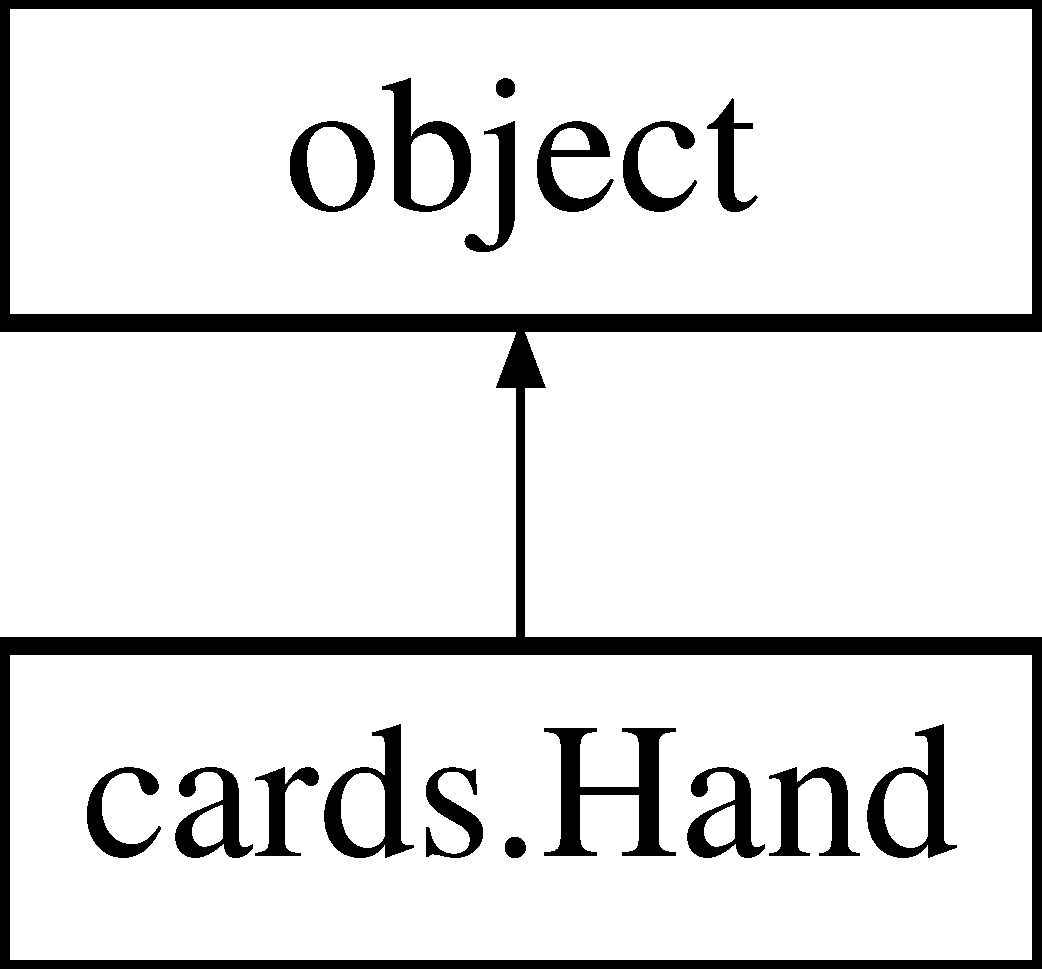
\includegraphics[height=2.000000cm]{classcards_1_1Hand}
\end{center}
\end{figure}
\subsection*{Public Member Functions}
\begin{DoxyCompactItemize}
\item 
def \hyperlink{classcards_1_1Hand_af800ad698281536204b51b71fb8ed15d}{\+\_\+\+\_\+init\+\_\+\+\_\+} (self, cards)
\item 
def \hyperlink{classcards_1_1Hand_a69f3ca64f85f68517e1aff96eecddf88}{n\+\_\+of\+\_\+a\+\_\+kind} (self, n)
\item 
def \hyperlink{classcards_1_1Hand_a6f47baa991d8cbc19de475dedc913c5d}{royal\+\_\+flush} (self)
\item 
def \hyperlink{classcards_1_1Hand_a968d069f9496b9be0b776cf556c9cc3e}{straight\+\_\+flush} (self)
\item 
def \hyperlink{classcards_1_1Hand_a154a7212af3b6230948078e83a5522a3}{four\+\_\+of\+\_\+a\+\_\+kind} (self)
\item 
def \hyperlink{classcards_1_1Hand_aa884f0c9ac8cb9e0d525fa6dd5f3b468}{full\+\_\+house} (self)
\item 
def \hyperlink{classcards_1_1Hand_a82d4acb563e208e8622948b436eceb60}{flush} (self)
\item 
def \hyperlink{classcards_1_1Hand_a29d0bc084338ab312ad249dc33e2f957}{straight} (self)
\item 
def \hyperlink{classcards_1_1Hand_a38deb8800110f1077223a605e5096cf2}{three\+\_\+of\+\_\+a\+\_\+kind} (self)
\item 
def \hyperlink{classcards_1_1Hand_a4bc879b8db18b48d745aecac892fa79c}{two\+\_\+pairs} (self)
\item 
def \hyperlink{classcards_1_1Hand_a0b6c8668a89a95ee985f475ae5b6775a}{one\+\_\+pair} (self)
\item 
def \hyperlink{classcards_1_1Hand_a52b92cc78391802ad2b9182bc326a403}{value} (self)
\item 
def \hyperlink{classcards_1_1Hand_a42ceab50738615707ec65667d1802496}{scoring\+\_\+cards} (self, score)
\item 
def \hyperlink{classcards_1_1Hand_aabc65985f97f74cefd0b550c3f47e652}{break\+\_\+tie} (self, other)
\item 
def \hyperlink{classcards_1_1Hand_a82fa918741361692526417b3295242dc}{\+\_\+\+\_\+lt\+\_\+\+\_\+} (self, other)
\item 
def \hyperlink{classcards_1_1Hand_a817ee76b140e59bf5c1e933283e5fb52}{\+\_\+\+\_\+le\+\_\+\+\_\+} (self, other)
\item 
def \hyperlink{classcards_1_1Hand_a1db1734329cd4a3be5a51447a1431646}{\+\_\+\+\_\+eq\+\_\+\+\_\+} (self, other)
\item 
def \hyperlink{classcards_1_1Hand_a35a85437e077522eef6448c863b6e570}{\+\_\+\+\_\+ne\+\_\+\+\_\+} (self, other)
\item 
def \hyperlink{classcards_1_1Hand_ae7d4f7a7e165bef7f32d6ed4c1781e6f}{\+\_\+\+\_\+gt\+\_\+\+\_\+} (self, other)
\item 
def \hyperlink{classcards_1_1Hand_a5d7400b5ff312926a03526db90acc22d}{\+\_\+\+\_\+ge\+\_\+\+\_\+} (self, other)
\end{DoxyCompactItemize}


\subsection{Constructor \& Destructor Documentation}
\hypertarget{classcards_1_1Hand_af800ad698281536204b51b71fb8ed15d}{}\index{cards\+::\+Hand@{cards\+::\+Hand}!\+\_\+\+\_\+init\+\_\+\+\_\+@{\+\_\+\+\_\+init\+\_\+\+\_\+}}
\index{\+\_\+\+\_\+init\+\_\+\+\_\+@{\+\_\+\+\_\+init\+\_\+\+\_\+}!cards\+::\+Hand@{cards\+::\+Hand}}
\subsubsection[{\+\_\+\+\_\+init\+\_\+\+\_\+}]{\setlength{\rightskip}{0pt plus 5cm}def cards.\+Hand.\+\_\+\+\_\+init\+\_\+\+\_\+ (
\begin{DoxyParamCaption}
\item[{}]{self, }
\item[{}]{cards}
\end{DoxyParamCaption}
)}\label{classcards_1_1Hand_af800ad698281536204b51b71fb8ed15d}


\subsection{Member Function Documentation}
\hypertarget{classcards_1_1Hand_a1db1734329cd4a3be5a51447a1431646}{}\index{cards\+::\+Hand@{cards\+::\+Hand}!\+\_\+\+\_\+eq\+\_\+\+\_\+@{\+\_\+\+\_\+eq\+\_\+\+\_\+}}
\index{\+\_\+\+\_\+eq\+\_\+\+\_\+@{\+\_\+\+\_\+eq\+\_\+\+\_\+}!cards\+::\+Hand@{cards\+::\+Hand}}
\subsubsection[{\+\_\+\+\_\+eq\+\_\+\+\_\+}]{\setlength{\rightskip}{0pt plus 5cm}def cards.\+Hand.\+\_\+\+\_\+eq\+\_\+\+\_\+ (
\begin{DoxyParamCaption}
\item[{}]{self, }
\item[{}]{other}
\end{DoxyParamCaption}
)}\label{classcards_1_1Hand_a1db1734329cd4a3be5a51447a1431646}
\hypertarget{classcards_1_1Hand_a5d7400b5ff312926a03526db90acc22d}{}\index{cards\+::\+Hand@{cards\+::\+Hand}!\+\_\+\+\_\+ge\+\_\+\+\_\+@{\+\_\+\+\_\+ge\+\_\+\+\_\+}}
\index{\+\_\+\+\_\+ge\+\_\+\+\_\+@{\+\_\+\+\_\+ge\+\_\+\+\_\+}!cards\+::\+Hand@{cards\+::\+Hand}}
\subsubsection[{\+\_\+\+\_\+ge\+\_\+\+\_\+}]{\setlength{\rightskip}{0pt plus 5cm}def cards.\+Hand.\+\_\+\+\_\+ge\+\_\+\+\_\+ (
\begin{DoxyParamCaption}
\item[{}]{self, }
\item[{}]{other}
\end{DoxyParamCaption}
)}\label{classcards_1_1Hand_a5d7400b5ff312926a03526db90acc22d}
\hypertarget{classcards_1_1Hand_ae7d4f7a7e165bef7f32d6ed4c1781e6f}{}\index{cards\+::\+Hand@{cards\+::\+Hand}!\+\_\+\+\_\+gt\+\_\+\+\_\+@{\+\_\+\+\_\+gt\+\_\+\+\_\+}}
\index{\+\_\+\+\_\+gt\+\_\+\+\_\+@{\+\_\+\+\_\+gt\+\_\+\+\_\+}!cards\+::\+Hand@{cards\+::\+Hand}}
\subsubsection[{\+\_\+\+\_\+gt\+\_\+\+\_\+}]{\setlength{\rightskip}{0pt plus 5cm}def cards.\+Hand.\+\_\+\+\_\+gt\+\_\+\+\_\+ (
\begin{DoxyParamCaption}
\item[{}]{self, }
\item[{}]{other}
\end{DoxyParamCaption}
)}\label{classcards_1_1Hand_ae7d4f7a7e165bef7f32d6ed4c1781e6f}
\hypertarget{classcards_1_1Hand_a817ee76b140e59bf5c1e933283e5fb52}{}\index{cards\+::\+Hand@{cards\+::\+Hand}!\+\_\+\+\_\+le\+\_\+\+\_\+@{\+\_\+\+\_\+le\+\_\+\+\_\+}}
\index{\+\_\+\+\_\+le\+\_\+\+\_\+@{\+\_\+\+\_\+le\+\_\+\+\_\+}!cards\+::\+Hand@{cards\+::\+Hand}}
\subsubsection[{\+\_\+\+\_\+le\+\_\+\+\_\+}]{\setlength{\rightskip}{0pt plus 5cm}def cards.\+Hand.\+\_\+\+\_\+le\+\_\+\+\_\+ (
\begin{DoxyParamCaption}
\item[{}]{self, }
\item[{}]{other}
\end{DoxyParamCaption}
)}\label{classcards_1_1Hand_a817ee76b140e59bf5c1e933283e5fb52}
\hypertarget{classcards_1_1Hand_a82fa918741361692526417b3295242dc}{}\index{cards\+::\+Hand@{cards\+::\+Hand}!\+\_\+\+\_\+lt\+\_\+\+\_\+@{\+\_\+\+\_\+lt\+\_\+\+\_\+}}
\index{\+\_\+\+\_\+lt\+\_\+\+\_\+@{\+\_\+\+\_\+lt\+\_\+\+\_\+}!cards\+::\+Hand@{cards\+::\+Hand}}
\subsubsection[{\+\_\+\+\_\+lt\+\_\+\+\_\+}]{\setlength{\rightskip}{0pt plus 5cm}def cards.\+Hand.\+\_\+\+\_\+lt\+\_\+\+\_\+ (
\begin{DoxyParamCaption}
\item[{}]{self, }
\item[{}]{other}
\end{DoxyParamCaption}
)}\label{classcards_1_1Hand_a82fa918741361692526417b3295242dc}
\hypertarget{classcards_1_1Hand_a35a85437e077522eef6448c863b6e570}{}\index{cards\+::\+Hand@{cards\+::\+Hand}!\+\_\+\+\_\+ne\+\_\+\+\_\+@{\+\_\+\+\_\+ne\+\_\+\+\_\+}}
\index{\+\_\+\+\_\+ne\+\_\+\+\_\+@{\+\_\+\+\_\+ne\+\_\+\+\_\+}!cards\+::\+Hand@{cards\+::\+Hand}}
\subsubsection[{\+\_\+\+\_\+ne\+\_\+\+\_\+}]{\setlength{\rightskip}{0pt plus 5cm}def cards.\+Hand.\+\_\+\+\_\+ne\+\_\+\+\_\+ (
\begin{DoxyParamCaption}
\item[{}]{self, }
\item[{}]{other}
\end{DoxyParamCaption}
)}\label{classcards_1_1Hand_a35a85437e077522eef6448c863b6e570}
\hypertarget{classcards_1_1Hand_aabc65985f97f74cefd0b550c3f47e652}{}\index{cards\+::\+Hand@{cards\+::\+Hand}!break\+\_\+tie@{break\+\_\+tie}}
\index{break\+\_\+tie@{break\+\_\+tie}!cards\+::\+Hand@{cards\+::\+Hand}}
\subsubsection[{break\+\_\+tie}]{\setlength{\rightskip}{0pt plus 5cm}def cards.\+Hand.\+break\+\_\+tie (
\begin{DoxyParamCaption}
\item[{}]{self, }
\item[{}]{other}
\end{DoxyParamCaption}
)}\label{classcards_1_1Hand_aabc65985f97f74cefd0b550c3f47e652}
\hypertarget{classcards_1_1Hand_a82d4acb563e208e8622948b436eceb60}{}\index{cards\+::\+Hand@{cards\+::\+Hand}!flush@{flush}}
\index{flush@{flush}!cards\+::\+Hand@{cards\+::\+Hand}}
\subsubsection[{flush}]{\setlength{\rightskip}{0pt plus 5cm}def cards.\+Hand.\+flush (
\begin{DoxyParamCaption}
\item[{}]{self}
\end{DoxyParamCaption}
)}\label{classcards_1_1Hand_a82d4acb563e208e8622948b436eceb60}
\hypertarget{classcards_1_1Hand_a154a7212af3b6230948078e83a5522a3}{}\index{cards\+::\+Hand@{cards\+::\+Hand}!four\+\_\+of\+\_\+a\+\_\+kind@{four\+\_\+of\+\_\+a\+\_\+kind}}
\index{four\+\_\+of\+\_\+a\+\_\+kind@{four\+\_\+of\+\_\+a\+\_\+kind}!cards\+::\+Hand@{cards\+::\+Hand}}
\subsubsection[{four\+\_\+of\+\_\+a\+\_\+kind}]{\setlength{\rightskip}{0pt plus 5cm}def cards.\+Hand.\+four\+\_\+of\+\_\+a\+\_\+kind (
\begin{DoxyParamCaption}
\item[{}]{self}
\end{DoxyParamCaption}
)}\label{classcards_1_1Hand_a154a7212af3b6230948078e83a5522a3}
\hypertarget{classcards_1_1Hand_aa884f0c9ac8cb9e0d525fa6dd5f3b468}{}\index{cards\+::\+Hand@{cards\+::\+Hand}!full\+\_\+house@{full\+\_\+house}}
\index{full\+\_\+house@{full\+\_\+house}!cards\+::\+Hand@{cards\+::\+Hand}}
\subsubsection[{full\+\_\+house}]{\setlength{\rightskip}{0pt plus 5cm}def cards.\+Hand.\+full\+\_\+house (
\begin{DoxyParamCaption}
\item[{}]{self}
\end{DoxyParamCaption}
)}\label{classcards_1_1Hand_aa884f0c9ac8cb9e0d525fa6dd5f3b468}
\hypertarget{classcards_1_1Hand_a69f3ca64f85f68517e1aff96eecddf88}{}\index{cards\+::\+Hand@{cards\+::\+Hand}!n\+\_\+of\+\_\+a\+\_\+kind@{n\+\_\+of\+\_\+a\+\_\+kind}}
\index{n\+\_\+of\+\_\+a\+\_\+kind@{n\+\_\+of\+\_\+a\+\_\+kind}!cards\+::\+Hand@{cards\+::\+Hand}}
\subsubsection[{n\+\_\+of\+\_\+a\+\_\+kind}]{\setlength{\rightskip}{0pt plus 5cm}def cards.\+Hand.\+n\+\_\+of\+\_\+a\+\_\+kind (
\begin{DoxyParamCaption}
\item[{}]{self, }
\item[{}]{n}
\end{DoxyParamCaption}
)}\label{classcards_1_1Hand_a69f3ca64f85f68517e1aff96eecddf88}
\hypertarget{classcards_1_1Hand_a0b6c8668a89a95ee985f475ae5b6775a}{}\index{cards\+::\+Hand@{cards\+::\+Hand}!one\+\_\+pair@{one\+\_\+pair}}
\index{one\+\_\+pair@{one\+\_\+pair}!cards\+::\+Hand@{cards\+::\+Hand}}
\subsubsection[{one\+\_\+pair}]{\setlength{\rightskip}{0pt plus 5cm}def cards.\+Hand.\+one\+\_\+pair (
\begin{DoxyParamCaption}
\item[{}]{self}
\end{DoxyParamCaption}
)}\label{classcards_1_1Hand_a0b6c8668a89a95ee985f475ae5b6775a}
\hypertarget{classcards_1_1Hand_a6f47baa991d8cbc19de475dedc913c5d}{}\index{cards\+::\+Hand@{cards\+::\+Hand}!royal\+\_\+flush@{royal\+\_\+flush}}
\index{royal\+\_\+flush@{royal\+\_\+flush}!cards\+::\+Hand@{cards\+::\+Hand}}
\subsubsection[{royal\+\_\+flush}]{\setlength{\rightskip}{0pt plus 5cm}def cards.\+Hand.\+royal\+\_\+flush (
\begin{DoxyParamCaption}
\item[{}]{self}
\end{DoxyParamCaption}
)}\label{classcards_1_1Hand_a6f47baa991d8cbc19de475dedc913c5d}
\hypertarget{classcards_1_1Hand_a42ceab50738615707ec65667d1802496}{}\index{cards\+::\+Hand@{cards\+::\+Hand}!scoring\+\_\+cards@{scoring\+\_\+cards}}
\index{scoring\+\_\+cards@{scoring\+\_\+cards}!cards\+::\+Hand@{cards\+::\+Hand}}
\subsubsection[{scoring\+\_\+cards}]{\setlength{\rightskip}{0pt plus 5cm}def cards.\+Hand.\+scoring\+\_\+cards (
\begin{DoxyParamCaption}
\item[{}]{self, }
\item[{}]{score}
\end{DoxyParamCaption}
)}\label{classcards_1_1Hand_a42ceab50738615707ec65667d1802496}
\hypertarget{classcards_1_1Hand_a29d0bc084338ab312ad249dc33e2f957}{}\index{cards\+::\+Hand@{cards\+::\+Hand}!straight@{straight}}
\index{straight@{straight}!cards\+::\+Hand@{cards\+::\+Hand}}
\subsubsection[{straight}]{\setlength{\rightskip}{0pt plus 5cm}def cards.\+Hand.\+straight (
\begin{DoxyParamCaption}
\item[{}]{self}
\end{DoxyParamCaption}
)}\label{classcards_1_1Hand_a29d0bc084338ab312ad249dc33e2f957}
\hypertarget{classcards_1_1Hand_a968d069f9496b9be0b776cf556c9cc3e}{}\index{cards\+::\+Hand@{cards\+::\+Hand}!straight\+\_\+flush@{straight\+\_\+flush}}
\index{straight\+\_\+flush@{straight\+\_\+flush}!cards\+::\+Hand@{cards\+::\+Hand}}
\subsubsection[{straight\+\_\+flush}]{\setlength{\rightskip}{0pt plus 5cm}def cards.\+Hand.\+straight\+\_\+flush (
\begin{DoxyParamCaption}
\item[{}]{self}
\end{DoxyParamCaption}
)}\label{classcards_1_1Hand_a968d069f9496b9be0b776cf556c9cc3e}
\hypertarget{classcards_1_1Hand_a38deb8800110f1077223a605e5096cf2}{}\index{cards\+::\+Hand@{cards\+::\+Hand}!three\+\_\+of\+\_\+a\+\_\+kind@{three\+\_\+of\+\_\+a\+\_\+kind}}
\index{three\+\_\+of\+\_\+a\+\_\+kind@{three\+\_\+of\+\_\+a\+\_\+kind}!cards\+::\+Hand@{cards\+::\+Hand}}
\subsubsection[{three\+\_\+of\+\_\+a\+\_\+kind}]{\setlength{\rightskip}{0pt plus 5cm}def cards.\+Hand.\+three\+\_\+of\+\_\+a\+\_\+kind (
\begin{DoxyParamCaption}
\item[{}]{self}
\end{DoxyParamCaption}
)}\label{classcards_1_1Hand_a38deb8800110f1077223a605e5096cf2}
\hypertarget{classcards_1_1Hand_a4bc879b8db18b48d745aecac892fa79c}{}\index{cards\+::\+Hand@{cards\+::\+Hand}!two\+\_\+pairs@{two\+\_\+pairs}}
\index{two\+\_\+pairs@{two\+\_\+pairs}!cards\+::\+Hand@{cards\+::\+Hand}}
\subsubsection[{two\+\_\+pairs}]{\setlength{\rightskip}{0pt plus 5cm}def cards.\+Hand.\+two\+\_\+pairs (
\begin{DoxyParamCaption}
\item[{}]{self}
\end{DoxyParamCaption}
)}\label{classcards_1_1Hand_a4bc879b8db18b48d745aecac892fa79c}
\hypertarget{classcards_1_1Hand_a52b92cc78391802ad2b9182bc326a403}{}\index{cards\+::\+Hand@{cards\+::\+Hand}!value@{value}}
\index{value@{value}!cards\+::\+Hand@{cards\+::\+Hand}}
\subsubsection[{value}]{\setlength{\rightskip}{0pt plus 5cm}def cards.\+Hand.\+value (
\begin{DoxyParamCaption}
\item[{}]{self}
\end{DoxyParamCaption}
)}\label{classcards_1_1Hand_a52b92cc78391802ad2b9182bc326a403}


The documentation for this class was generated from the following file\+:\begin{DoxyCompactItemize}
\item 
\hyperlink{cards_8py}{cards.\+py}\end{DoxyCompactItemize}

\chapter{File Documentation}
\hypertarget{cards_8py}{}\section{cards.\+py File Reference}
\label{cards_8py}\index{cards.\+py@{cards.\+py}}
\subsection*{Classes}
\begin{DoxyCompactItemize}
\item 
class \hyperlink{classcards_1_1Hand}{cards.\+Hand}
\end{DoxyCompactItemize}
\subsection*{Namespaces}
\begin{DoxyCompactItemize}
\item 
 \hyperlink{namespacecards}{cards}
\end{DoxyCompactItemize}
\subsection*{Functions}
\begin{DoxyCompactItemize}
\item 
def \hyperlink{namespacecards_ab58172fe17df72a0805b634ba5ec70fc}{cards.\+cards\+\_\+cmp} (a, b)
\item 
def \hyperlink{namespacecards_aca908702299162f0ce7ebed192ae90b2}{cards.\+denom} (card)
\end{DoxyCompactItemize}

\hypertarget{combinatorics_8py}{}\section{combinatorics.\+py File Reference}
\label{combinatorics_8py}\index{combinatorics.\+py@{combinatorics.\+py}}
\subsection*{Namespaces}
\begin{DoxyCompactItemize}
\item 
 \hyperlink{namespacecombinatorics}{combinatorics}
\end{DoxyCompactItemize}
\subsection*{Functions}
\begin{DoxyCompactItemize}
\item 
def \hyperlink{namespacecombinatorics_af4ad63ab1a68ba7c7efe8751623bc187}{combinatorics.\+fib} (n)
\item 
def \hyperlink{namespacecombinatorics_a14c14265f587c6fd4fc1bb9829ff5504}{combinatorics.\+digits} (n)
\item 
def \hyperlink{namespacecombinatorics_a37b7002188355ef3cac6f40cadb915ff}{combinatorics.\+nub} (nums)
\item 
def \hyperlink{namespacecombinatorics_a20423365036ac6b3e8560c994273e448}{combinatorics.\+has\+\_\+square} (n)
\end{DoxyCompactItemize}

\hypertarget{primes_8py}{}\section{primes.\+py File Reference}
\label{primes_8py}\index{primes.\+py@{primes.\+py}}
\subsection*{Namespaces}
\begin{DoxyCompactItemize}
\item 
 \hyperlink{namespaceprimes}{primes}
\end{DoxyCompactItemize}
\subsection*{Functions}
\begin{DoxyCompactItemize}
\item 
def \hyperlink{namespaceprimes_a27386dc3226d6aa9ec6ae476753d176f}{primes.\+primes\+\_\+seq} (n)
\item 
def \hyperlink{namespaceprimes_a7dffa5a7e9ee87a726e91e03a673282d}{primes.\+is\+\_\+next\+\_\+prime} (n, sieve)
\item 
def \hyperlink{namespaceprimes_a42460a84d6704d490f48e32fb5e5de66}{primes.\+is\+\_\+prime} (n, sieve)
\item 
def \hyperlink{namespaceprimes_a0fc2c4db3043a8d17dbd564ed9a3335e}{primes.\+next\+\_\+prime} (sieve)
\item 
def \hyperlink{namespaceprimes_afc18a8897a2405ada153fc92e27b4322}{primes.\+primes}
\item 
def \hyperlink{namespaceprimes_ae0a9ada316f92cba9ef0bad5495314fb}{primes.\+odd\+\_\+composite} ()
\item 
def \hyperlink{namespaceprimes_a8d1a9642a31428d166fdc5a8e400ce2a}{primes.\+factors} (n)
\end{DoxyCompactItemize}

%--- End generated contents ---

% Index
\backmatter
\newpage
\phantomsection
\clearemptydoublepage
\addcontentsline{toc}{chapter}{Index}
\printindex

\end{document}
